\documentclass{standalone}
\usepackage{tikz}
\usetikzlibrary{patterns, positioning}


\begin{document}
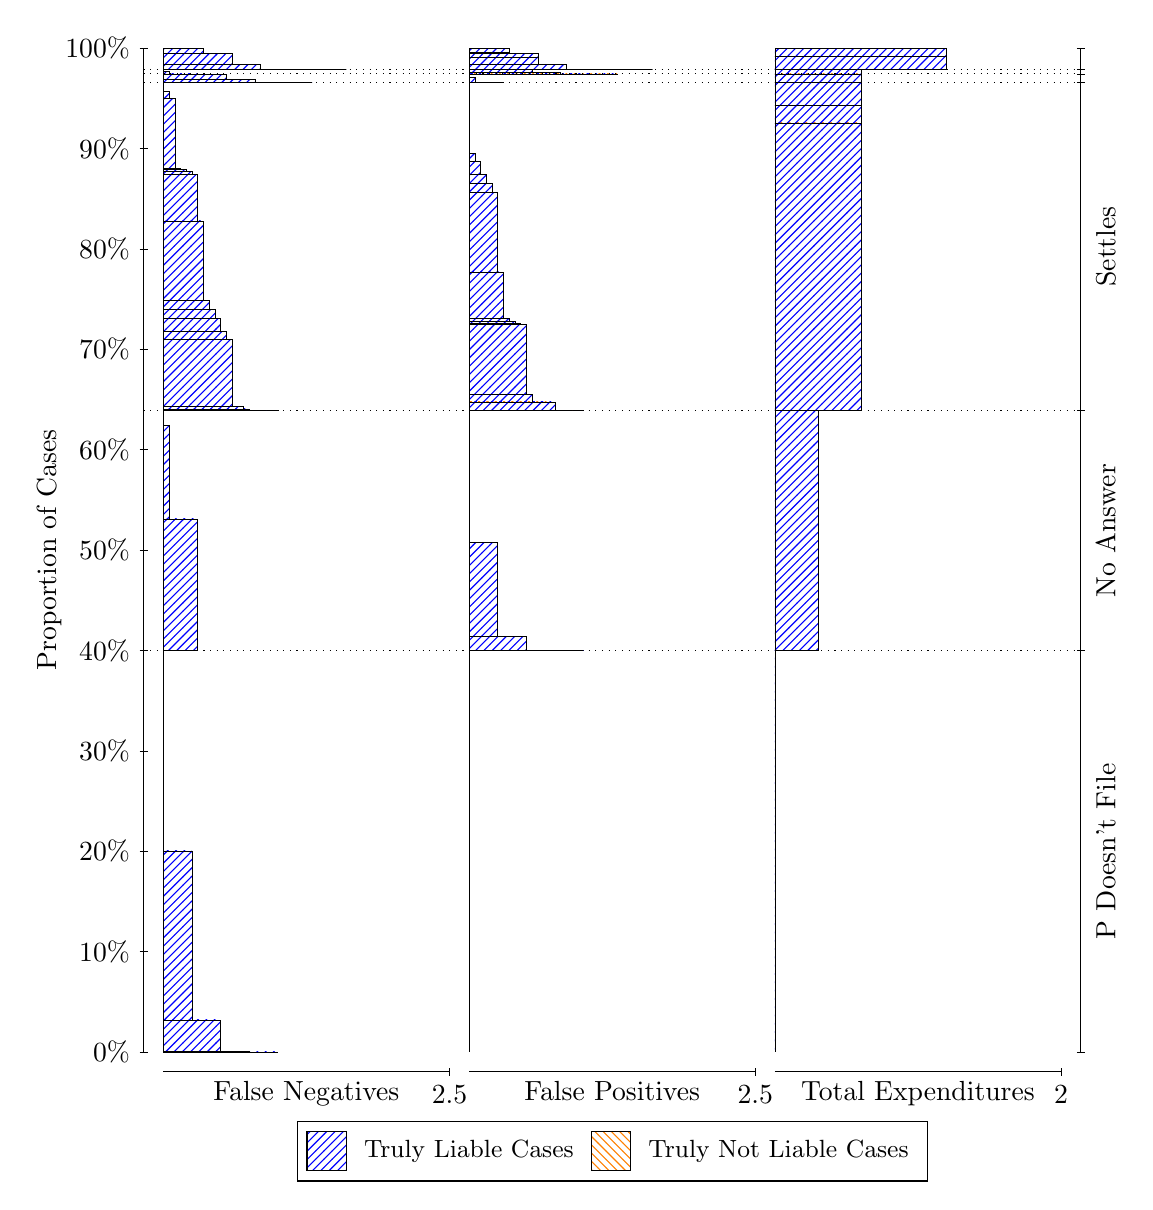
\begin{tikzpicture}
\draw[black, very thin] (1.5,1.75) -- (1.5,14.5);
\node[rotate=90, text=black, anchor=center] at (0.3, 8.125) {Proportion of Cases};
\draw[black, very thin] (1.45,1.75) -- (1.55,1.75);
\node[text=black, anchor=east] at (1.45, 1.75) {0\%};
\draw[black, very thin] (1.45,3.025) -- (1.55,3.025);
\node[text=black, anchor=east] at (1.45, 3.025) {10\%};
\draw[black, very thin] (1.45,4.3) -- (1.55,4.3);
\node[text=black, anchor=east] at (1.45, 4.3) {20\%};
\draw[black, very thin] (1.45,5.575) -- (1.55,5.575);
\node[text=black, anchor=east] at (1.45, 5.575) {30\%};
\draw[black, very thin] (1.45,6.85) -- (1.55,6.85);
\node[text=black, anchor=east] at (1.45, 6.85) {40\%};
\draw[black, very thin] (1.45,8.125) -- (1.55,8.125);
\node[text=black, anchor=east] at (1.45, 8.125) {50\%};
\draw[black, very thin] (1.45,9.4) -- (1.55,9.4);
\node[text=black, anchor=east] at (1.45, 9.4) {60\%};
\draw[black, very thin] (1.45,10.675) -- (1.55,10.675);
\node[text=black, anchor=east] at (1.45, 10.675) {70\%};
\draw[black, very thin] (1.45,11.95) -- (1.55,11.95);
\node[text=black, anchor=east] at (1.45, 11.95) {80\%};
\draw[black, very thin] (1.45,13.225) -- (1.55,13.225);
\node[text=black, anchor=east] at (1.45, 13.225) {90\%};
\draw[black, very thin] (1.45,14.5) -- (1.55,14.5);
\node[text=black, anchor=east] at (1.45, 14.5) {100\%};

\draw[black, very thin] (13.4,1.75) -- (13.4,14.5);
\draw[black, very thin] (13.35,1.75) -- (13.45,1.75);
\node[anchor=west] at (13.35, 1.75) {};
\draw[black, very thin] (13.35,6.8489) -- (13.45,6.8489);
\node[anchor=west] at (13.35, 6.8489) {};
\draw[black, very thin] (13.35,9.8947) -- (13.45,9.8947);
\node[anchor=west] at (13.35, 9.8947) {};
\draw[black, very thin] (13.35,14.067) -- (13.45,14.067);
\node[anchor=west] at (13.35, 14.067) {};
\draw[black, very thin] (13.35,14.171) -- (13.45,14.171);
\node[anchor=west] at (13.35, 14.171) {};
\draw[black, very thin] (13.35,14.226) -- (13.45,14.226);
\node[anchor=west] at (13.35, 14.226) {};
\draw[black, very thin] (13.35,14.5) -- (13.45,14.5);
\node[anchor=west] at (13.35, 14.5) {};

\draw[black, very thin, pattern color=blue, pattern=north east lines] (1.75,1.75) rectangle (3.2033,1.75);
\draw[black, very thin, pattern color=blue, pattern=north east lines] (1.75,1.75) rectangle (2.84,1.7534);
\draw[black, very thin, pattern color=blue, pattern=north east lines] (1.75,1.7534) rectangle (2.4767,2.158);
\draw[black, very thin, pattern color=blue, pattern=north east lines] (1.75,2.158) rectangle (2.1133,4.3029);
\draw[black, very thin, pattern color=orange, pattern=north west lines] (1.75,4.3029) rectangle (1.75,4.3029);
\draw[black, very thin, pattern color=blue, pattern=north east lines] (1.75,4.3029) rectangle (1.75,6.8489);
\draw[black, very thin, pattern color=blue, pattern=north east lines] (1.75,6.8489) rectangle (2.186,8.5202);
\draw[black, very thin, pattern color=blue, pattern=north east lines] (1.75,8.5202) rectangle (1.8227,9.7143);
\draw[black, very thin, pattern color=orange, pattern=north west lines] (1.75,9.7143) rectangle (1.75,9.7143);
\draw[black, very thin, pattern color=blue, pattern=north east lines] (1.75,9.7143) rectangle (1.75,9.8947);
\draw[black, very thin, pattern color=blue, pattern=north east lines] (1.75,9.8947) rectangle (3.2033,9.8948);
\draw[black, very thin, pattern color=blue, pattern=north east lines] (1.75,9.8948) rectangle (3.058,9.8948);
\draw[black, very thin, pattern color=blue, pattern=north east lines] (1.75,9.8948) rectangle (2.9127,9.895);
\draw[black, very thin, pattern color=blue, pattern=north east lines] (1.75,9.895) rectangle (2.84,9.9174);
\draw[black, very thin, pattern color=blue, pattern=north east lines] (1.75,9.9174) rectangle (2.7673,9.9462);
\draw[black, very thin, pattern color=blue, pattern=north east lines] (1.75,9.9462) rectangle (2.6947,9.952);
\draw[black, very thin, pattern color=blue, pattern=north east lines] (1.75,9.952) rectangle (2.622,10.799);
\draw[black, very thin, pattern color=blue, pattern=north east lines] (1.75,10.799) rectangle (2.5493,10.905);
\draw[black, very thin, pattern color=blue, pattern=north east lines] (1.75,10.905) rectangle (2.4767,11.065);
\draw[black, very thin, pattern color=blue, pattern=north east lines] (1.75,11.065) rectangle (2.404,11.183);
\draw[black, very thin, pattern color=blue, pattern=north east lines] (1.75,11.183) rectangle (2.3313,11.291);
\draw[black, very thin, pattern color=blue, pattern=north east lines] (1.75,11.291) rectangle (2.2587,12.304);
\draw[black, very thin, pattern color=blue, pattern=north east lines] (1.75,12.304) rectangle (2.186,12.894);
\draw[black, very thin, pattern color=blue, pattern=north east lines] (1.75,12.894) rectangle (2.1133,12.932);
\draw[black, very thin, pattern color=blue, pattern=north east lines] (1.75,12.932) rectangle (2.0407,12.961);
\draw[black, very thin, pattern color=blue, pattern=north east lines] (1.75,12.961) rectangle (1.968,12.967);
\draw[black, very thin, pattern color=blue, pattern=north east lines] (1.75,12.967) rectangle (1.8953,13.865);
\draw[black, very thin, pattern color=blue, pattern=north east lines] (1.75,13.865) rectangle (1.8227,13.954);
\draw[black, very thin, pattern color=orange, pattern=north west lines] (1.75,13.954) rectangle (1.75,13.954);
\draw[black, very thin, pattern color=blue, pattern=north east lines] (1.75,13.954) rectangle (1.75,14.067);
\draw[black, very thin, pattern color=blue, pattern=north east lines] (1.75,14.067) rectangle (3.6393,14.067);
\draw[black, very thin, pattern color=blue, pattern=north east lines] (1.75,14.067) rectangle (3.276,14.067);
\draw[black, very thin, pattern color=blue, pattern=north east lines] (1.75,14.067) rectangle (2.9127,14.106);
\draw[black, very thin, pattern color=blue, pattern=north east lines] (1.75,14.106) rectangle (2.5493,14.17);
\draw[black, very thin, pattern color=blue, pattern=north east lines] (1.75,14.17) rectangle (2.186,14.171);
\draw[black, very thin, pattern color=orange, pattern=north west lines] (1.75,14.171) rectangle (1.75,14.171);
\draw[black, very thin, pattern color=blue, pattern=north east lines] (1.75,14.171) rectangle (2.186,14.172);
\draw[black, very thin, pattern color=blue, pattern=north east lines] (1.75,14.172) rectangle (1.8227,14.206);
\draw[black, very thin, pattern color=orange, pattern=north west lines] (1.75,14.206) rectangle (1.75,14.206);
\draw[black, very thin, pattern color=blue, pattern=north east lines] (1.75,14.206) rectangle (1.75,14.226);
\draw[black, very thin, pattern color=blue, pattern=north east lines] (1.75,14.226) rectangle (4.0753,14.226);
\draw[black, very thin, pattern color=blue, pattern=north east lines] (1.75,14.226) rectangle (3.712,14.227);
\draw[black, very thin, pattern color=blue, pattern=north east lines] (1.75,14.227) rectangle (3.3487,14.23);
\draw[black, very thin, pattern color=blue, pattern=north east lines] (1.75,14.23) rectangle (2.9853,14.294);
\draw[black, very thin, pattern color=blue, pattern=north east lines] (1.75,14.294) rectangle (2.622,14.431);
\draw[black, very thin, pattern color=blue, pattern=north east lines] (1.75,14.431) rectangle (2.2587,14.495);
\draw[black, very thin, pattern color=blue, pattern=north east lines] (1.75,14.495) rectangle (1.8953,14.5);
\draw[black, very thin, pattern color=orange, pattern=north west lines] (1.75,14.5) rectangle (1.75,14.5);
\draw[black, very thin, pattern color=blue, pattern=north east lines] (1.75,14.5) rectangle (1.75,14.5);
\draw[black, very thin, pattern color=orange, pattern=north west lines] (5.6333,1.75) rectangle (5.6333,1.75);
\draw[black, very thin, pattern color=blue, pattern=north east lines] (5.6333,1.75) rectangle (5.6333,6.8489);
\draw[black, very thin, pattern color=orange, pattern=north west lines] (5.6333,6.8489) rectangle (7.0867,6.8489);
\draw[black, very thin, pattern color=blue, pattern=north east lines] (5.6333,6.8489) rectangle (7.0867,6.8489);
\draw[black, very thin, pattern color=blue, pattern=north east lines] (5.6333,6.8489) rectangle (6.7233,6.8491);
\draw[black, very thin, pattern color=blue, pattern=north east lines] (5.6333,6.8491) rectangle (6.36,7.0293);
\draw[black, very thin, pattern color=blue, pattern=north east lines] (5.6333,7.0293) rectangle (5.9967,8.2234);
\draw[black, very thin, pattern color=blue, pattern=north east lines] (5.6333,8.2234) rectangle (5.6333,9.8947);
\draw[black, very thin, pattern color=orange, pattern=north west lines] (5.6333,9.8947) rectangle (7.0867,9.8947);
\draw[black, very thin, pattern color=blue, pattern=north east lines] (5.6333,9.8947) rectangle (7.0867,9.895);
\draw[black, very thin, pattern color=orange, pattern=north west lines] (5.6333,9.895) rectangle (6.9413,9.895);
\draw[black, very thin, pattern color=blue, pattern=north east lines] (5.6333,9.895) rectangle (6.9413,9.895);
\draw[black, very thin, pattern color=orange, pattern=north west lines] (5.6333,9.895) rectangle (6.796,9.895);
\draw[black, very thin, pattern color=blue, pattern=north east lines] (5.6333,9.895) rectangle (6.796,9.8952);
\draw[black, very thin, pattern color=blue, pattern=north east lines] (5.6333,9.8952) rectangle (6.7233,10.007);
\draw[black, very thin, pattern color=orange, pattern=north west lines] (5.6333,10.007) rectangle (6.6507,10.007);
\draw[black, very thin, pattern color=blue, pattern=north east lines] (5.6333,10.007) rectangle (6.6507,10.007);
\draw[black, very thin, pattern color=blue, pattern=north east lines] (5.6333,10.007) rectangle (6.578,10.007);
\draw[black, very thin, pattern color=orange, pattern=north west lines] (5.6333,10.007) rectangle (6.5053,10.007);
\draw[black, very thin, pattern color=blue, pattern=north east lines] (5.6333,10.007) rectangle (6.5053,10.007);
\draw[black, very thin, pattern color=blue, pattern=north east lines] (5.6333,10.007) rectangle (6.4327,10.097);
\draw[black, very thin, pattern color=blue, pattern=north east lines] (5.6333,10.097) rectangle (6.36,10.995);
\draw[black, very thin, pattern color=blue, pattern=north east lines] (5.6333,10.995) rectangle (6.2873,11);
\draw[black, very thin, pattern color=blue, pattern=north east lines] (5.6333,11) rectangle (6.2147,11.029);
\draw[black, very thin, pattern color=blue, pattern=north east lines] (5.6333,11.029) rectangle (6.142,11.068);
\draw[black, very thin, pattern color=blue, pattern=north east lines] (5.6333,11.068) rectangle (6.0693,11.658);
\draw[black, very thin, pattern color=blue, pattern=north east lines] (5.6333,11.658) rectangle (5.9967,12.67);
\draw[black, very thin, pattern color=blue, pattern=north east lines] (5.6333,12.67) rectangle (5.924,12.778);
\draw[black, very thin, pattern color=blue, pattern=north east lines] (5.6333,12.778) rectangle (5.8513,12.897);
\draw[black, very thin, pattern color=blue, pattern=north east lines] (5.6333,12.897) rectangle (5.7787,13.057);
\draw[black, very thin, pattern color=blue, pattern=north east lines] (5.6333,13.057) rectangle (5.706,13.162);
\draw[black, very thin, pattern color=blue, pattern=north east lines] (5.6333,13.162) rectangle (5.6333,14.067);
\draw[black, very thin, pattern color=orange, pattern=north west lines] (5.6333,14.067) rectangle (6.0693,14.067);
\draw[black, very thin, pattern color=blue, pattern=north east lines] (5.6333,14.067) rectangle (6.0693,14.068);
\draw[black, very thin, pattern color=blue, pattern=north east lines] (5.6333,14.068) rectangle (5.706,14.132);
\draw[black, very thin, pattern color=blue, pattern=north east lines] (5.6333,14.132) rectangle (5.6333,14.171);
\draw[black, very thin, pattern color=orange, pattern=north west lines] (5.6333,14.171) rectangle (7.5227,14.171);
\draw[black, very thin, pattern color=blue, pattern=north east lines] (5.6333,14.171) rectangle (7.5227,14.171);
\draw[black, very thin, pattern color=blue, pattern=north east lines] (5.6333,14.171) rectangle (7.1593,14.171);
\draw[black, very thin, pattern color=blue, pattern=north east lines] (5.6333,14.171) rectangle (6.796,14.192);
\draw[black, very thin, pattern color=blue, pattern=north east lines] (5.6333,14.192) rectangle (6.4327,14.226);
\draw[black, very thin, pattern color=blue, pattern=north east lines] (5.6333,14.226) rectangle (6.0693,14.226);
\draw[black, very thin, pattern color=orange, pattern=north west lines] (5.6333,14.226) rectangle (7.9587,14.226);
\draw[black, very thin, pattern color=blue, pattern=north east lines] (5.6333,14.226) rectangle (7.9587,14.226);
\draw[black, very thin, pattern color=orange, pattern=north west lines] (5.6333,14.226) rectangle (7.5953,14.226);
\draw[black, very thin, pattern color=blue, pattern=north east lines] (5.6333,14.226) rectangle (7.5953,14.227);
\draw[black, very thin, pattern color=orange, pattern=north west lines] (5.6333,14.227) rectangle (7.232,14.227);
\draw[black, very thin, pattern color=blue, pattern=north east lines] (5.6333,14.227) rectangle (7.232,14.231);
\draw[black, very thin, pattern color=blue, pattern=north east lines] (5.6333,14.231) rectangle (6.8687,14.294);
\draw[black, very thin, pattern color=orange, pattern=north west lines] (5.6333,14.294) rectangle (6.8687,14.294);
\draw[black, very thin, pattern color=blue, pattern=north east lines] (5.6333,14.294) rectangle (6.8687,14.295);
\draw[black, very thin, pattern color=blue, pattern=north east lines] (5.6333,14.295) rectangle (6.5053,14.383);
\draw[black, very thin, pattern color=orange, pattern=north west lines] (5.6333,14.383) rectangle (6.5053,14.383);
\draw[black, very thin, pattern color=blue, pattern=north east lines] (5.6333,14.383) rectangle (6.5053,14.433);
\draw[black, very thin, pattern color=blue, pattern=north east lines] (5.6333,14.433) rectangle (6.142,14.446);
\draw[black, very thin, pattern color=blue, pattern=north east lines] (5.6333,14.446) rectangle (6.142,14.496);
\draw[black, very thin, pattern color=blue, pattern=north east lines] (5.6333,14.496) rectangle (5.7787,14.496);
\draw[black, very thin, pattern color=blue, pattern=north east lines] (5.6333,14.496) rectangle (5.7787,14.5);
\draw[black, very thin, pattern color=blue, pattern=north east lines] (5.6333,14.5) rectangle (5.6333,14.5);
\draw[black, very thin, pattern color=orange, pattern=north west lines] (9.5167,1.75) rectangle (9.5167,1.75);
\draw[black, very thin, pattern color=blue, pattern=north east lines] (9.5167,1.75) rectangle (9.5167,6.8489);
\draw[black, very thin, pattern color=orange, pattern=north west lines] (9.5167,6.8489) rectangle (10.062,6.8489);
\draw[black, very thin, pattern color=blue, pattern=north east lines] (9.5167,6.8489) rectangle (10.062,9.8947);
\draw[black, very thin, pattern color=orange, pattern=north west lines] (9.5167,9.8947) rectangle (10.607,9.8947);
\draw[black, very thin, pattern color=blue, pattern=north east lines] (9.5167,9.8947) rectangle (10.607,13.55);
\draw[black, very thin, pattern color=orange, pattern=north west lines] (9.5167,13.55) rectangle (10.607,13.55);
\draw[black, very thin, pattern color=blue, pattern=north east lines] (9.5167,13.55) rectangle (10.607,13.771);
\draw[black, very thin, pattern color=orange, pattern=north west lines] (9.5167,13.771) rectangle (10.607,13.771);
\draw[black, very thin, pattern color=blue, pattern=north east lines] (9.5167,13.771) rectangle (10.607,14.067);
\draw[black, very thin, pattern color=orange, pattern=north west lines] (9.5167,14.067) rectangle (10.607,14.067);
\draw[black, very thin, pattern color=blue, pattern=north east lines] (9.5167,14.067) rectangle (10.607,14.171);
\draw[black, very thin, pattern color=orange, pattern=north west lines] (9.5167,14.171) rectangle (10.607,14.171);
\draw[black, very thin, pattern color=blue, pattern=north east lines] (9.5167,14.171) rectangle (10.607,14.226);
\draw[black, very thin, pattern color=orange, pattern=north west lines] (9.5167,14.226) rectangle (11.697,14.226);
\draw[black, very thin, pattern color=blue, pattern=north east lines] (9.5167,14.226) rectangle (11.697,14.396);
\draw[black, very thin, pattern color=orange, pattern=north west lines] (9.5167,14.396) rectangle (11.697,14.396);
\draw[black, very thin, pattern color=blue, pattern=north east lines] (9.5167,14.396) rectangle (11.697,14.5);
\draw[black, dotted] (1.5,6.8489) -- (13.4,6.8489);
\draw[black, dotted] (1.5,9.8947) -- (13.4,9.8947);
\draw[black, dotted] (1.5,14.067) -- (13.4,14.067);
\draw[black, dotted] (1.5,14.171) -- (13.4,14.171);
\draw[black, dotted] (1.5,14.226) -- (13.4,14.226);
\draw[black, very thin] (1.75,1.5) -- (5.3833,1.5);
\node[text=black, anchor=north] at (3.5667, 1.5) {False Negatives};
\draw[black, very thin] (5.3833,1.45) -- (5.3833,1.55);
\node[text=black, anchor=north] at (5.3833, 1.45) {2.5};

\draw[black, very thin] (5.6333,1.5) -- (9.2667,1.5);
\node[text=black, anchor=north] at (7.45, 1.5) {False Positives};
\draw[black, very thin] (9.2667,1.45) -- (9.2667,1.55);
\node[text=black, anchor=north] at (9.2667, 1.45) {2.5};

\draw[black, very thin] (9.5167,1.5) -- (13.15,1.5);
\node[text=black, anchor=north] at (11.333, 1.5) {Total Expenditures};
\draw[black, very thin] (13.15,1.45) -- (13.15,1.55);
\node[text=black, anchor=north] at (13.15, 1.45) {2};

\node[text=black, centered, rotate=90] at (13.72, 4.2994) {P Doesn't File};
\node[text=black, centered, rotate=90] at (13.72, 8.3718) {No Answer};
\node[text=black, centered, rotate=90] at (13.72, 11.981) {Settles};




\draw (7.449999999999999,1.5) node[draw=none] (baseCoordinate) {};
\begin{scope}[align=center]
        \matrix[scale=0.5, draw=black, below=0.5cm of baseCoordinate, nodes={draw}, column sep=0.1cm]{
            \node[rectangle, draw, minimum width=0.5cm, minimum height=0.5cm, pattern color=blue, pattern=north east lines] {}; &
            \node[draw=none, font=\small, text=black] (B) {Truly Liable Cases}; &
            \node[rectangle, draw, minimum width=0.5cm, minimum height=0.5cm, pattern color=orange, pattern=north west lines] {}; &
            \node[draw=none, font=\small, text=black] (B) {Truly Not Liable Cases}; \\
            };
\end{scope}

\end{tikzpicture}
\end{document}